\documentclass{article}
\usepackage[utf8]{inputenc}
\usepackage{graphicx}


\renewcommand{\vec}[1]{
	\mathbf{#1}
}


\title{Machine Learning Algorithms}
\date{\today}

\begin{document}
	
	\maketitle
	
	\section*{Linear Regression}
	
	We assume the the target variable $t$ is given by the form:
	\[t = \vec{w}\cdot\vec{x} + \epsilon \]
	where $\epsilon$ is a zero mean Gaussian random variable with variance $\sigma$. The probability distribution for the target variable $t$ is given by 
	\[p(t|\vec{x}, \vec{w}, \sigma) = \mathcal{N}( t| \vec{w}\cdot \vec{x}, \sigma)\]
	This is probability for single instance in the dataset.	
	
	% ADD MAXIMUM LIKELYHOOD DERIVATION
	
	% ADD SHOW DERIVATION OF NORMAL EQUATION FROM LEAST SQUARES COST
	\begin{figure}
		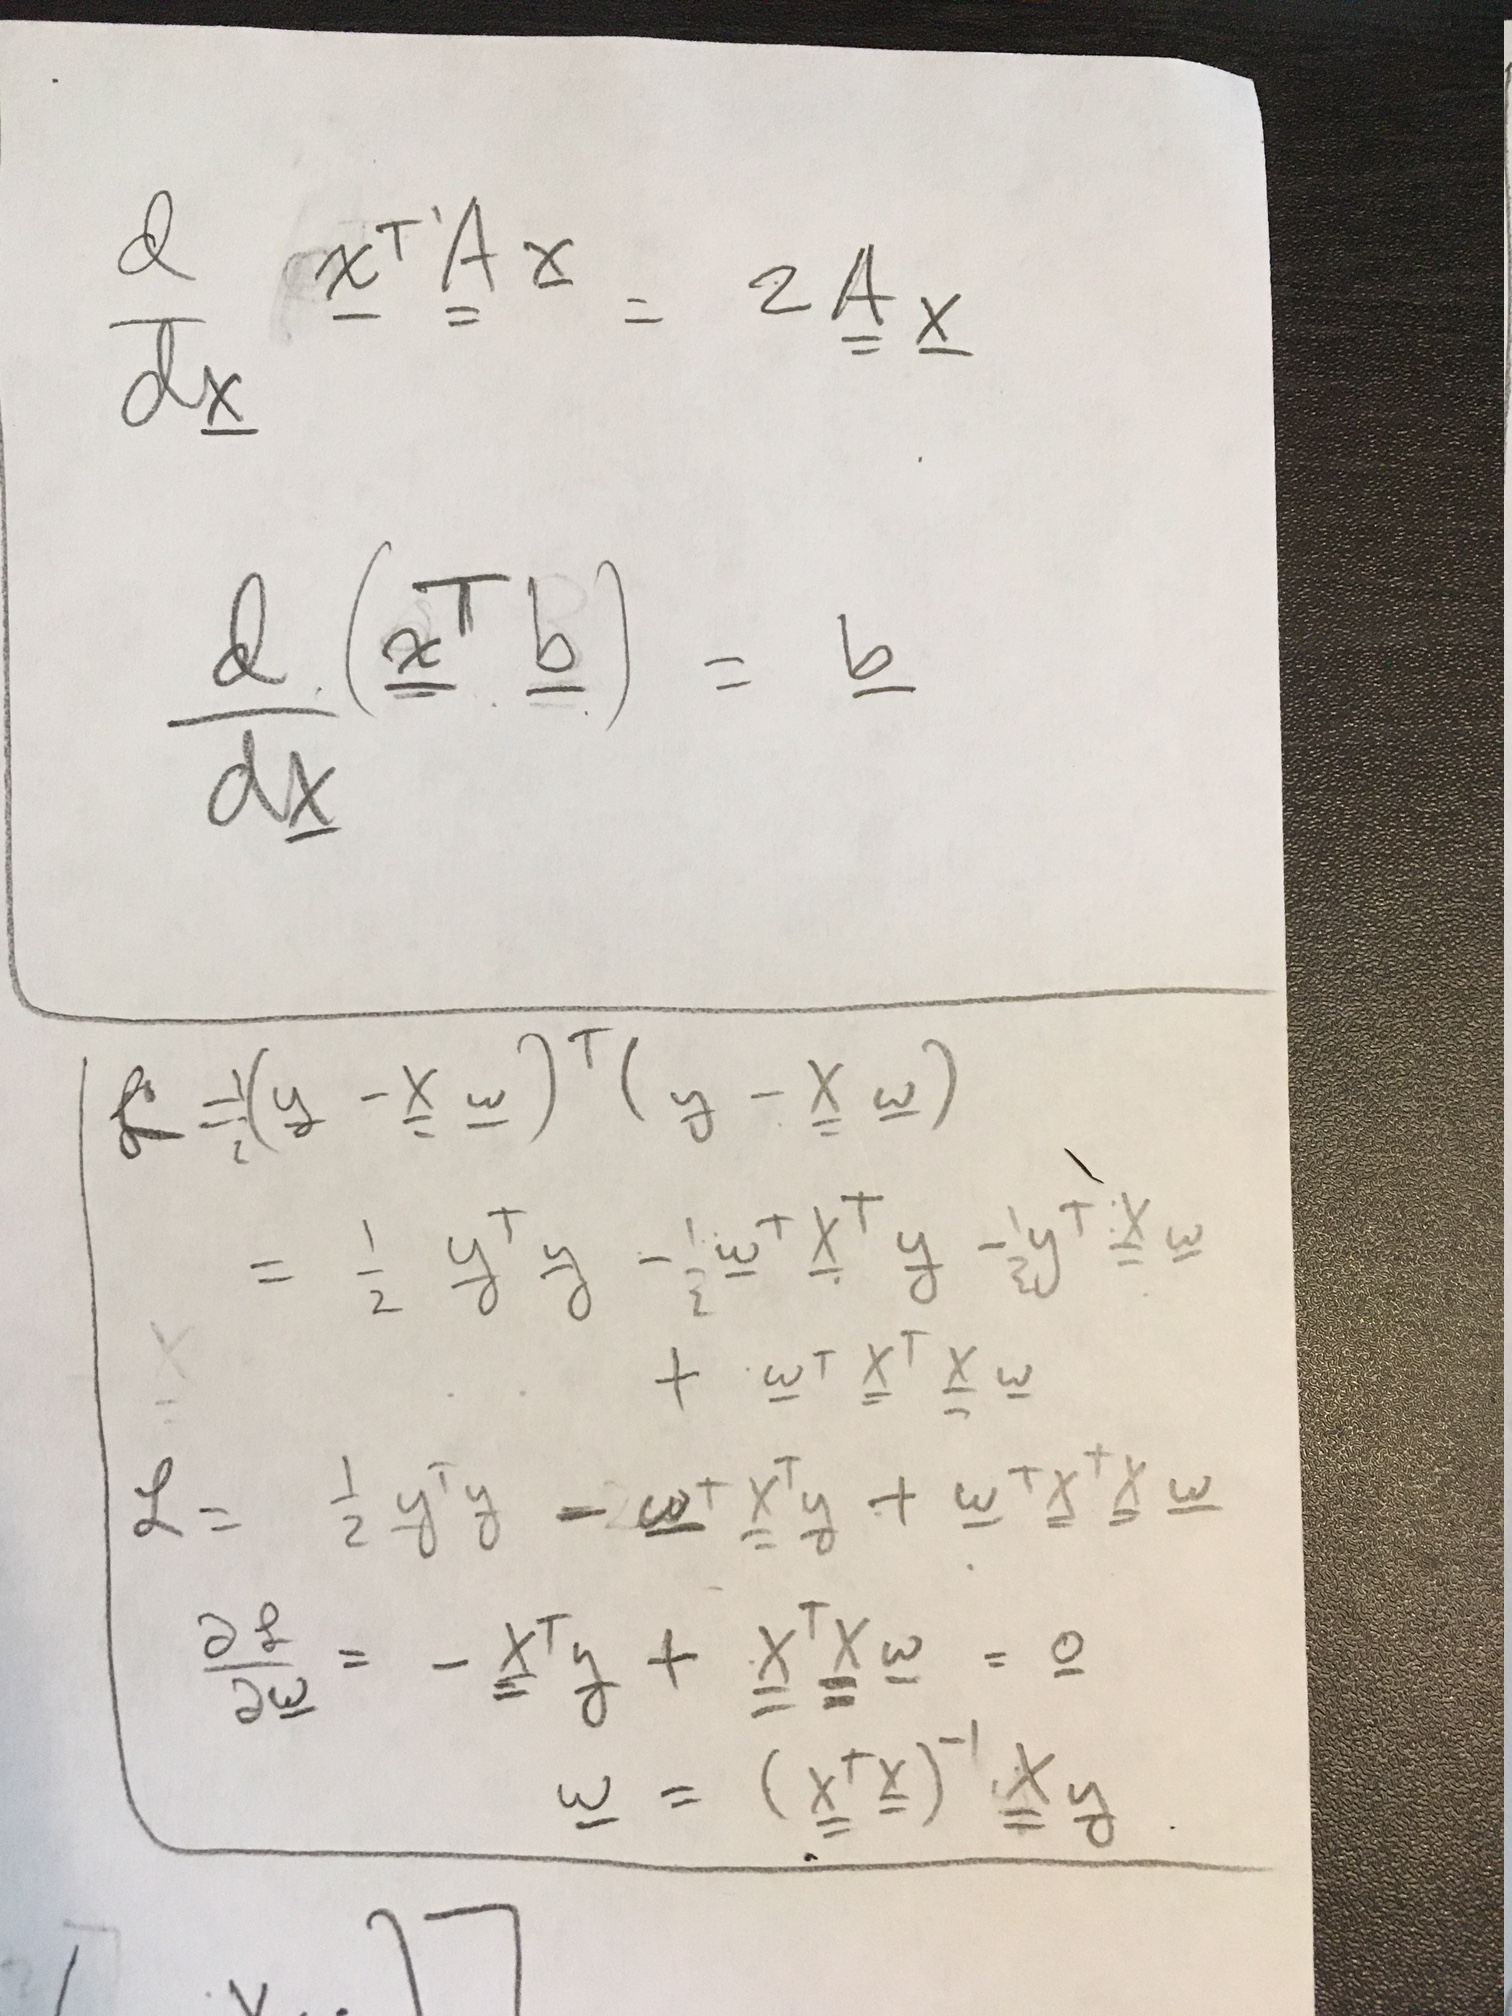
\includegraphics[width=0.5\textwidth]{images/linear-regression-normal-equation}
	\end{figure}
	
	Normal equation is given by:

	\[\vec{w} = (\vec{X}^T\vec{X})^{-1}\vec{X}^T\vec{y}\]
    \section*{Logistic Regression}
	
	\section*{SVM}
	
	\section*{Tree-Based Methods}
	
	\section*{Random Forest}
	
	\section*{K-nearest Neighbors}
	
	\section*{K-means Clustering}
	
	\section*{Probabilistic Graphical Models}
	
	\section*{Markov Models}
	
	\section*{PCA / SVD}
	
	\section*{Fully Connected Neural Networks}
	
	\section*{Convolutional Neural Networks}
	
	\section*{Recurrent Neural Networks}
	
	\section*{Transformers}	
	
	\section*{ARIMA}
	
	\section*{Reinforcement Learning}
	
	\section*{Deep Q Learning}
	
	\section*{PPO}
	
\end{document}